\chapter{从意图到运动}\label{ch:g12:brain-and-movement}

一位女士某天清晨醒来，发现右臂和右腿无法活动，
却仍然有感觉；医生叩击她的右膝时，
膝跳\omterm{def:g12:stretch-reflex:reflex}{反射}比以往更加剧烈。扫描显示，她的大脑左半球
靠近顶部处有一小块坏死区域。其下的一切——神经、
脊髓、上一章的\omterm{def:g12:stretch-reflex:reflex}{反射弧}、肌肉——都完好无损，
但运动的意图却无法传达到它们。经过六个月的康复训练，
她重新能够行走，而她大脑工作时的扫描图像显示，
一些此前并不支配腿部的区域开始亮起。本章追踪一次随意运动
从皮层到运动\omterm{def:g12:stretch-reflex:neuron}{神经元}的路径，
并说明支配这一运动的“地图”如何被绘制、交叉，
再被重新绘制。

\section{运动皮层}

\begin{definition}[运动皮层]\label{def:g12:brain-and-movement:cortex}
\emph{初级运动皮层}\index{初级运动皮层}是覆盖在每个大脑半球顶部的一条
皮层带，位于分隔额叶与顶叶的中央沟之前。
其\omterm{def:g12:stretch-reflex:neuron}{神经元}是随意运动的起点，它们的轴突穿过脑干与脊髓，
下行至支配肌肉的运动\omterm{def:g12:stretch-reflex:neuron}{神经元}。该皮层带是身体的一幅
\emph{地图}：每一部分支配身体的一个部位，
次序自半球顶部的足部，一直延伸到侧面的面部。
每一部分所占的面积
并不取决于身体部位的大小，
而取决于其运动的精细程度，
因此手和面部占据了其中的大部分。
\end{definition}

\begin{proposition}[定位图真实存在，且为交叉支配]\label{prop:g12:brain-and-movement:map}
以电流刺激运动皮层的某一点，
会引起身体对应部位在\emph{对侧}产生运动；
损伤该点则使该部位对侧的
随意运动丧失。
\end{proposition}
\begin{proof}[证据]
在局部麻醉下进行脑部手术时，彭菲尔德（20 世纪 30 年代）
对暴露的皮层各点施以微弱电流，并记录哪些肌肉发生运动：
这些点构成了上述地图，手和面部所占区域远超其实际大小，
且每一次运动都发生在被刺激半球的对侧。
对健康志愿者进行功能成像显示：移动一根手指时，
对侧半球中预测位置出现活动斑点；
移动足部时，斑点则位于半球顶部，
脑卒中损毁一侧运动皮层的部分区域，
使另一侧对应部位瘫痪，而感觉保持完好。
\end{proof}

\begin{omfigure}
\begin{tikzpicture}
  \node[anchor=south west, inner sep=0] (img) at (0,0)
    {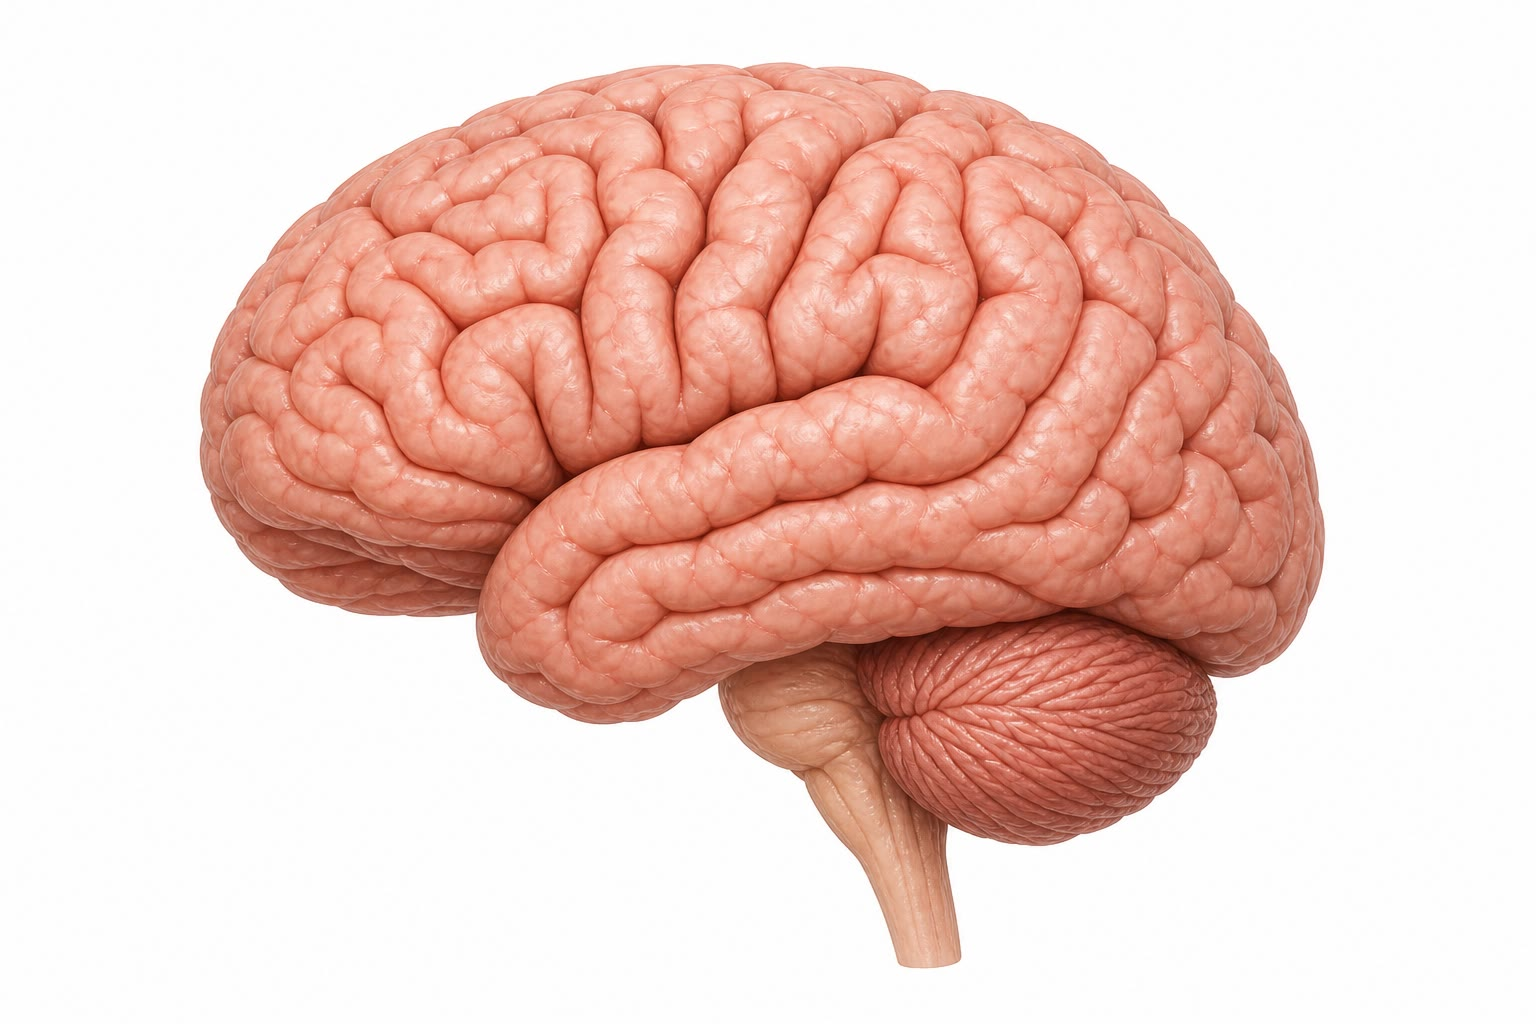
\includegraphics[width=0.52\linewidth]{images/book2/ai/fig-brain-side.jpg}};
  \begin{scope}[x={(img.south east)}, y={(img.north west)},
      every node/.style={font=\small}]
    \draw[omThm, very thick] (0.50,0.90) .. controls (0.53,0.75) .. (0.58,0.55);
    \draw[omDef, thick] (0.52,0.82) -- (0.45,1.08) node[above, align=center] {初级运动皮层 \\ （中央沟之前的皮层带）};
    \draw[omDef, thick] (0.28,0.72) -- (0.10,1.02) node[above] {额叶：规划};
    \draw[omDef, thick] (0.72,0.72) -- (0.85,1.02) node[above] {顶叶：感觉};
    \draw[omDef, thick] (0.70,0.28) -- (1.04,0.20) node[right] {小脑};
    \draw[omDef, thick] (0.60,0.10) -- (0.60,-0.06) node[below] {脑干：通路在此交叉};
  \end{scope}
\end{tikzpicture}

{\small 从左侧观察的大脑，\omterm{def:g12:brain-and-movement:cortex}{初级运动皮层}以红色标出：
这是位于半球顶部的一条皮层带，支配身体的右侧。
其下行纤维在脑干中交叉
至另一侧。}
\end{omfigure}

\begin{omfigure}
\begin{tikzpicture}
\begin{axis}[
  xbar, bar width=9pt,
  width=0.8\linewidth, height=6cm,
  axis x line=bottom, axis y line=left,
  xmin=0, xmax=35, xlabel={运动皮层所占份额（\%）},
  xlabel style={font=\small, at={(axis description cs:0.5,-0.1)}, anchor=north},
   symbolic y coords={toesfoot, leg, trunk, arm, handfingers, facetongue},
  ytick=data, yticklabels={脚趾和足, 腿, 躯干, 手臂, 手和手指, 面部和舌}, tick label style={font=\small},
  enlarge y limits=0.12, xtick={0,10,20,30},
  nodes near coords, nodes near coords style={font=\scriptsize, anchor=west},
]
\addplot[fill=omThm!50, draw=omThm] coordinates
   {(4,toesfoot) (8,leg) (6,trunk) (14,arm) (32,handfingers) (30,facetongue)};
\end{axis}
\end{tikzpicture}

{\small 各身体部位在运动皮层中所占份额的近似值。手和面部
运动最为精细，合计占据近三分之二；躯干运动较少，
仅占二十分之一。面积取决于精细程度，
而非身体大小。}
\end{omfigure}

\begin{omfigure}
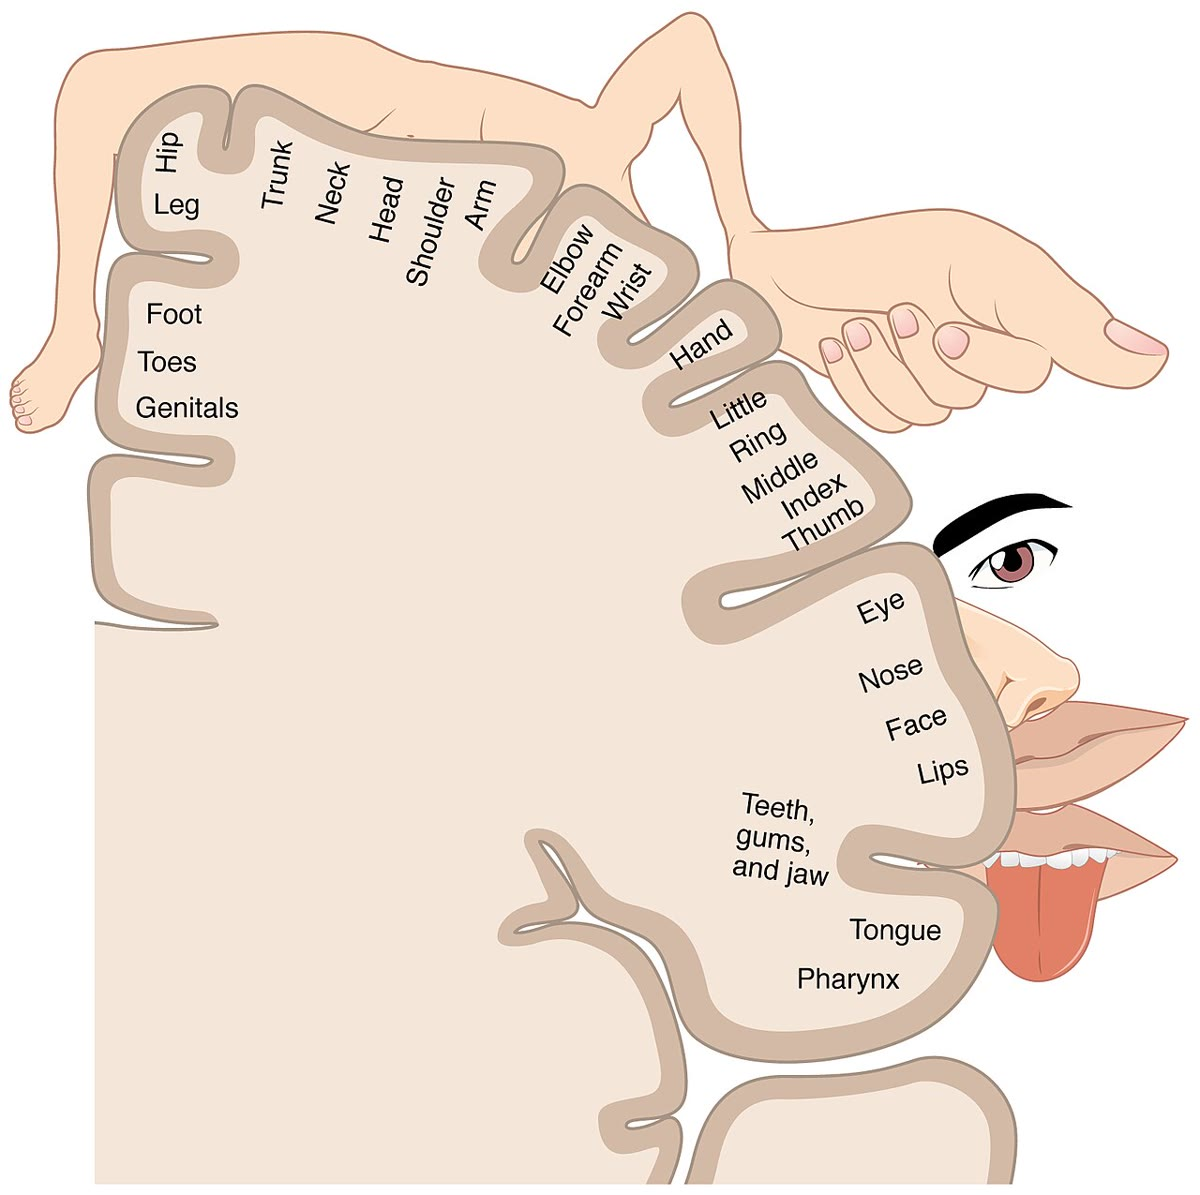
\includegraphics[width=0.5\linewidth]{images/book2/homunculus.jpg}

{\small 将地图画成人体：各部位的大小按其所占的皮层面积绘制，叠加在大脑半球的一个切面上。这是紧邻运动皮层之后的感觉皮层带；运动地图的排列顺序与之相同，比例也几乎一致——手和面部极大，躯干和腿部较小。插图来自 OpenStax《解剖学与生理学》，CC~BY~3.0。}
\end{omfigure}

\section{下行通路}

\begin{proposition}[从皮层到运动神经元]\label{prop:g12:brain-and-movement:pathway}
运动皮层\omterm{def:g12:stretch-reflex:neuron}{神经元}的轴突构成\emph{皮质脊髓
束}\index{皮质脊髓束}。该束穿过脑干下行，
其中大部分纤维在此交叉至另一侧——
这正是每侧大脑半球支配身体对侧的原因——并沿脊髓继续下行，
在每一节段，纤维分出并止于该节段肌肉的运动\omterm{def:g12:stretch-reflex:neuron}{神经元}，
或止于其旁的中间\omterm{def:g12:stretch-reflex:neuron}{神经元}。
因此，\cref{ch:g12:stretch-reflex}中的运动\omterm{def:g12:stretch-reflex:neuron}{神经元}
是两条指令的交汇点：一条来自肌梭、属于\omterm{def:g12:stretch-reflex:reflex}{反射弧}的指令，
另一条来自皮层，位于上方约一米处。
\end{proposition}
\begin{proof}[证据]
沿皮层经脑干追踪纤维，可观察到交叉现象；
位于交叉之上的束受损，使对侧瘫痪；
位于交叉之下的束受损，则使同侧瘫痪。
脊髓损伤会使损伤平面以下两侧的一切运动丧失，
而面部得以保留，因其纤维在上方离开束路；
损伤平面以下的\omterm{def:g12:stretch-reflex:reflex}{反射}依然存在，因其\omterm{def:g12:stretch-reflex:reflex}{反射弧}完好，
并且增强，因为皮层的阻尼作用已无法到达这些部位。
\end{proof}

\begin{omfigure}
\begin{tikzpicture}[font=\small, >=Stealth, line cap=round]
  % left hemisphere box, brainstem, cord, muscles
  \draw[thick, fill=omDef!8, rounded corners=10pt] (-3.4,4.2) rectangle (-0.2,5.8);
  \node at (-1.8,5.0) {左侧运动皮层};
  \draw[thick, fill=omDef!8, rounded corners=10pt] (0.2,4.2) rectangle (3.4,5.8);
  \node at (1.8,5.0) {右侧运动皮层};
  \draw[thick, fill=gray!15] (-0.8,1.6) rectangle (0.8,3.6);
  \node[font=\scriptsize, anchor=east] at (-0.9,3.3) {脑干};
  \draw[thick, fill=gray!10] (-0.6,-2.4) rectangle (0.6,1.6);
  \node[font=\scriptsize, rotate=90] at (0,-0.4) {脊髓};
  % tracts: left cortex -> crosses -> right side of cord -> right muscles
  \draw[very thick, omThm] (-1.8,4.2) -- (-0.4,3.4) -- (-0.4,2.6) -- (0.35,2.0) -- (0.35,-1.6);
  \draw[very thick, omDef] (1.8,4.2) -- (0.4,3.4) -- (0.4,2.6) -- (-0.35,2.0) -- (-0.35,-1.6);
  \node[font=\scriptsize, anchor=west] at (0.9,2.3) {交叉};
  % motor neurons and muscles
  \fill[omThm] (0.35,-1.6) circle (2.5pt); \draw[very thick, omThm] (0.35,-1.6) -- (2.6,-1.6);
  \draw[thick, fill=omThm!25, rounded corners=5pt] (2.6,-2.0) rectangle (3.8,-1.2); \node[font=\scriptsize] at (3.2,-1.6) {右腿};
  \fill[omDef] (-0.35,-1.6) circle (2.5pt); \draw[very thick, omDef] (-0.35,-1.6) -- (-2.6,-1.6);
  \draw[thick, fill=omDef!25, rounded corners=5pt] (-3.8,-2.0) rectangle (-2.6,-1.2); \node[font=\scriptsize] at (-3.2,-1.6) {左腿};
  \node[font=\scriptsize, anchor=west, align=left] at (0.9,0.3) {运动神经元：皮层指令 \\与反射弧的汇合点};
  \draw[gray, thin] (0.9,-0.2) -- (0.5,-1.45);
  \draw[->, thick, gray] (3.2,-2.4) .. controls (2.0,-3.0) and (0.8,-2.6) .. (0.5,-1.8);
  \node[font=\scriptsize, gray, anchor=north] at (2.2,-2.8) {右腿肌梭（反射输入）};
\end{tikzpicture}

{\small \omterm{prop:g12:brain-and-movement:pathway}{皮质脊髓束}。来自左侧运动皮层的纤维
（红色）在脑干交叉，沿脊髓右侧下行至
右腿的运动\omterm{def:g12:stretch-reflex:neuron}{神经元}；右侧皮层（蓝色）支配
左侧。每个运动\omterm{def:g12:stretch-reflex:neuron}{神经元}还接受其所支配肌肉的
\omterm{def:g12:stretch-reflex:reflex}{反射}输入。}
\end{omfigure}

\begin{example}[解读瘫痪]\label{ex:g12:brain-and-movement:paralysis}
右臂和右腿瘫痪，面部也瘫痪，感觉保留：左侧大脑半球的运动皮层
或其在交叉以上的纤维受损——即开篇的那位女士。
双腿瘫痪，手臂和面部未受累，腿部\omterm{def:g12:stretch-reflex:reflex}{反射}增强：脊髓
在下背部水平受损。一条手臂松软无力，\omterm{def:g12:stretch-reflex:reflex}{反射}消失：
神经或运动\omterm{def:g12:stretch-reflex:neuron}{神经元}本身受损，其以下
已无从放电。
图谱、交叉与\omterm{def:g12:stretch-reflex:reflex}{反射弧}，在任何扫描之前
就能定位损伤。
\end{example}

\section{运动神经元作出决定}

\begin{proposition}[运动神经元上的整合]\label{prop:g12:brain-and-movement:integration}
一个运动\omterm{def:g12:stretch-reflex:neuron}{神经元}接收成千上万个\omterm{def:g12:stretch-reflex:synapse}{突触}：兴奋性\omterm{def:g12:stretch-reflex:synapse}{突触}来自
皮层和肌梭，抑制性\omterm{def:g12:stretch-reflex:synapse}{突触}来自中间\omterm{def:g12:stretch-reflex:neuron}{神经元}，
而这些中间\omterm{def:g12:stretch-reflex:neuron}{神经元}受拮抗肌的肌梭、皮层及其他
中枢驱动。每个到达的信号都使膜电位略有改变，
使其趋向或远离阈值；这些改变在毫秒内、沿\omterm{def:g10:cells-common-unit:cell}{细胞}表面
\emph{叠加}，只有总和越过阈值时\omterm{def:g12:stretch-reflex:neuron}{神经元}才放电。
因此，运动\omterm{def:g12:stretch-reflex:neuron}{神经元}并非中继站，而是一台计算器：
肌肉是否收缩，取决于到达运动\omterm{def:g12:stretch-reflex:neuron}{神经元}的
所有指令之间的平衡，这便是运动的
\emph{最后公路}\index{最后公路}。
\end{proposition}
\begin{proof}[证据]
在运动\omterm{def:g12:stretch-reflex:neuron}{神经元}内记录显示，每个兴奋性输入都使其产生一个
约一毫伏的小幅去极化，远低于所需的
\qty{15}{mV}；一串输入，或来自多个来源的输入同时到达，
叠加至阈值即产生\omterm{prop:g12:stretch-reflex:actionpotential}{动作电位}；同时到达的抑制性输入会
抵消一个兴奋性输入。随意收缩的强度随被募集的运动\omterm{def:g12:stretch-reflex:neuron}{神经元}
数目和放电频率的增加而增强；受试者紧握拳头时，
膝跳\omterm{def:g12:stretch-reflex:reflex}{反射}更强，
这正是皮层的兴奋
与肌梭的兴奋相加。
\end{proof}

\begin{omfigure}
\begin{tikzpicture}
\begin{axis}[
  width=0.9\linewidth, height=5.6cm,
  axis x line=bottom, axis y line=left,
  xmin=0, xmax=40, ymin=-80, ymax=40,
  xlabel={时间（ms）}, ylabel={运动神经元电压（mV）},
  xlabel style={font=\small, at={(axis description cs:0.5,-0.12)}, anchor=north},
  ylabel style={font=\small},
  tick label style={font=\small}, xtick={0,10,20,30,40}, ytick={-70,-55,0,30},
  clip=false,
]
\addplot[thick, omDef] coordinates {(0,-70) (5,-70) (5.5,-66) (8,-68) (10,-70) (14,-70) (14.5,-66) (16,-64) (17,-61) (18.5,-58) (19.5,-55) (20,-30) (20.5,30) (21,0) (21.5,-50) (22,-75) (25,-72) (28,-70) (30,-70) (30.5,-66) (31.5,-70) (32,-74) (34,-70) (40,-70)};
\draw[dashed, gray] (axis cs:0,-55) -- (axis cs:40,-55);
  \node[font=\scriptsize, gray, anchor=south west] at (axis cs:0.3,-55) {阈值};
  \node[font=\scriptsize, anchor=south] at (axis cs:9,-67.5) {一个兴奋性输入};
  \node[font=\scriptsize, anchor=south, align=center] at (axis cs:11.5,-45) {四个输入快速相继到达 \\总和达到阈值};
  \node[font=\scriptsize, anchor=south, align=center] at (axis cs:31,-58) {兴奋性 + 抑制性：\\相互抵消};
\end{axis}
\end{tikzpicture}

{\small 运动\omterm{def:g12:stretch-reflex:neuron}{神经元}的整合。单个兴奋性输入使其去极化数毫伏，随即消退；
若干在毫秒内相继到达的输入叠加至阈值，\omterm{def:g12:stretch-reflex:neuron}{神经元}便放电；
与兴奋性输入同时到达的抑制性输入会
将其抵消。}
\end{omfigure}

\begin{example}[端起一杯水]\label{ex:g12:brain-and-movement:glass}
端起一杯满满的水时，皮层向手臂的运动\omterm{def:g12:stretch-reflex:neuron}{神经元}
持续发送稳定的兴奋；杯子倾斜时被拉长的肌梭
也加入其中；动作过冲时，拮抗肌的中间\omterm{def:g12:stretch-reflex:neuron}{神经元}
进行抑制；小脑比较预期动作与实际动作，
在数十毫秒之后修正皮层的指令。每个运动\omterm{def:g12:stretch-reflex:neuron}{神经元}
综合全部这些信号，恰好放电即可。
动作的平稳，取决于各总和之间的平衡。
\end{example}

\section{可重绘的图谱}

\begin{proposition}[运动皮层的可塑性]\label{prop:g12:brain-and-movement:plasticity}
运动图谱并非固定不变。练习某一动作会扩大支配该动作的
皮层区域并强化其连接；肢体制动时，
该肢体对应的区域会缩小；截肢后，该区域
则由邻近部位接管。中风之后，损伤周围未受损的皮层，
以及对侧半球的对应区域，能够学会支配受累的肌肉——
前提是要加以使用：康复训练通过反复强制动作，
使保留下来的神经回路被选择并
得到强化。\cref{ch:g11:vision-and-brain}中讨论的可塑性
同样适用于大脑的指令端，
正如适用于感觉端一样。
\end{proposition}
\begin{proof}[证据]
对小提琴手的皮层进行成像显示，
左手手指对应的区域增大，且增大程度与开始练习的年龄有关；
普通志愿者练习一组手指动作五天后，
这些手指对应的区域可测得明显增大，
停止练习后又会缩小。中风后，
瘫痪的手臂若经过强化训练——约束健侧手臂——
其功能恢复优于依靠健侧手臂代偿的患者，
成像显示，恢复的动作由损伤附近的
区域支配。手指区域受损的猴子，
只有在手指得到锻炼时才能恢复手指运动。
\end{proof}

\begin{omfigure}
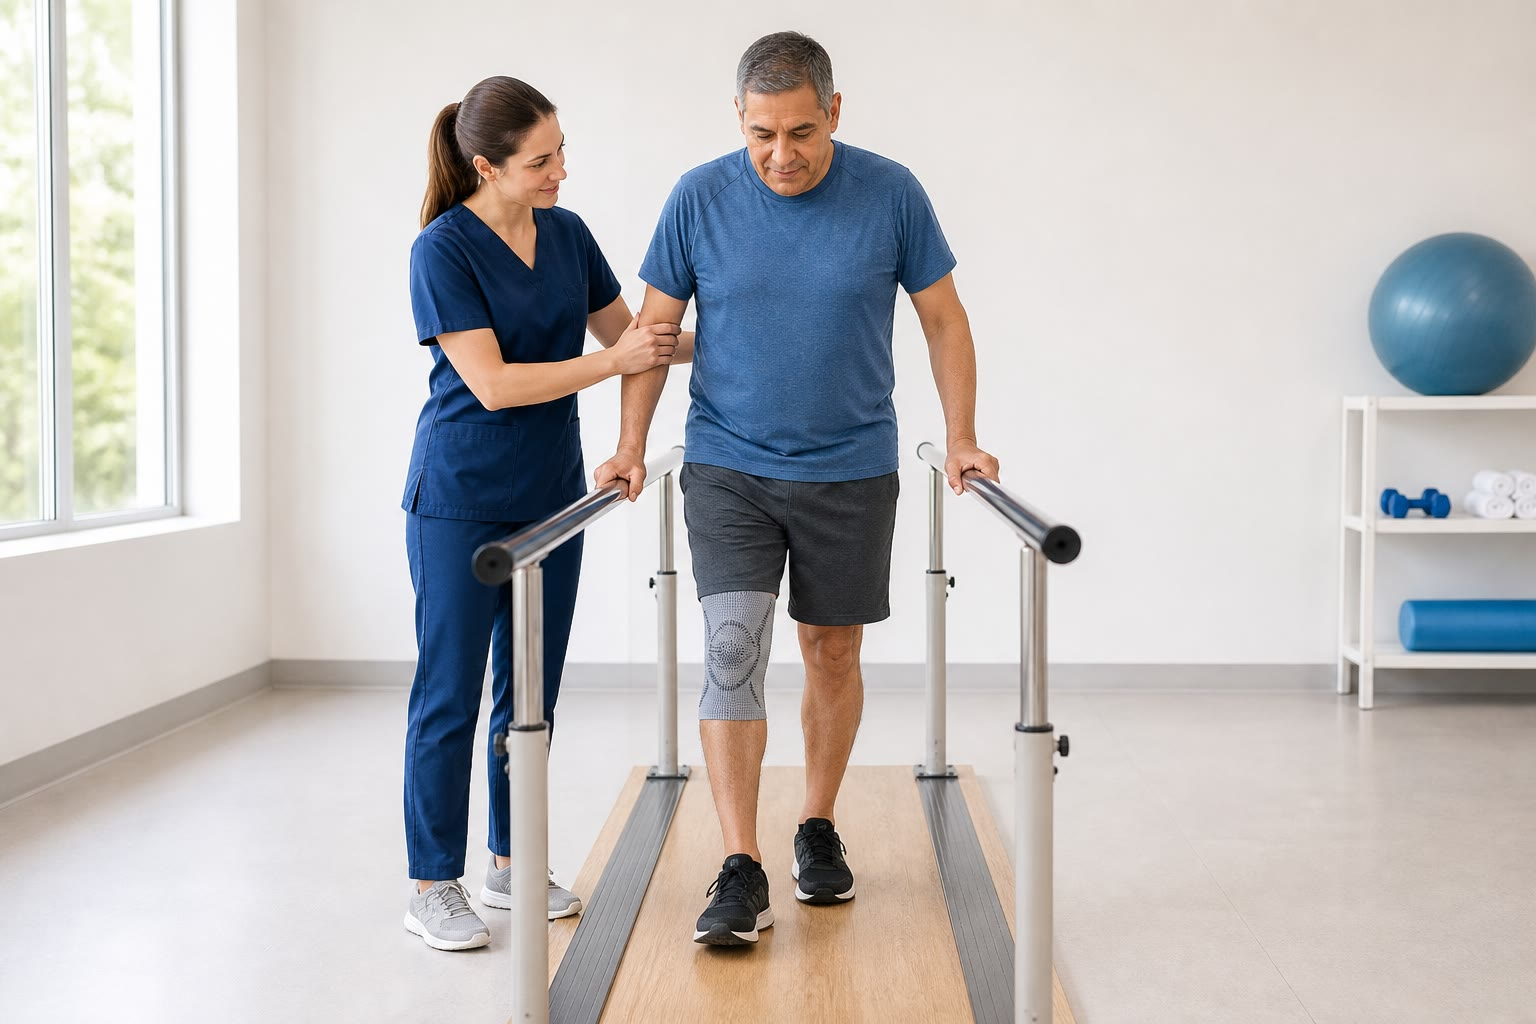
\includegraphics[width=0.56\linewidth]{images/book2/ai/g12-move-rehab.jpg}

{\small 中风后的康复：在平行杆之间
重新学习行走。每一次被迫迈出的步子，
都会筛选并强化仍能支配腿部的存活回路，
而皮层图谱会在损伤周围被重新绘制。}
\end{omfigure}

\begin{example}[中风六个月后]\label{ex:g12:brain-and-movement:sixmonths}
第 1 周：右腿不动；其\omterm{def:g12:stretch-reflex:reflex}{反射}亢进。
第 2--6 周：治疗师先移动腿部，再让患者尝试每个动作；
微弱的收缩重新出现。第 2--4 个月：
在平行杆之间行走，每天一千步；成像显示活动
在损伤周围的皮层及另一侧半球中扩散。
第 6 个月：拄着拐杖行走。损伤并未愈合
——皮层\omterm{def:g12:stretch-reflex:neuron}{神经元}不会再生——但邻近回路已被征召，
而恢复的每一步，
都是通过尝试该动作而完成的。
\end{example}

\begin{method}[定位运动障碍]\label{met:g12:brain-and-movement:locate}
\begin{enumerate}
  \item 哪些部位受累？身体一侧（包括面部）
        ：对侧半球或交叉以上的纤维。
        双侧以某一水平以下受累而面部不受累：该水平的脊髓。
        仅一个肢体或一组肌肉受累：其神经或
        运动\omterm{def:g12:stretch-reflex:neuron}{神经元}。
  \item \omterm{def:g12:stretch-reflex:reflex}{反射}是否保留？亢进：\omterm{def:g12:stretch-reflex:reflex}{反射弧}完整，
        皮层阻尼作用丧失（损伤位于运动\omterm{def:g12:stretch-reflex:neuron}{神经元}之上）。
        消失：\omterm{def:g12:stretch-reflex:reflex}{反射弧}本身中断（运动\omterm{def:g12:stretch-reflex:neuron}{神经元}，
        神经或肌肉）。
  \item 感觉是否保留？单纯运动缺损提示运动通路受损；
        运动与感觉同时受累，则提示两者均受影响的损伤。
  \item 能够恢复到什么程度？皮层损伤借助可塑性和训练，可以恢复；
        脊髓或神经离断，恢复空间小得多；肌肉和运动\omterm{def:g12:stretch-reflex:neuron}{神经元}疾病，
        视病因而定。
\end{enumerate}
\end{method}

\begin{remark}[一年中的最后一个回路]\label{rem:g12:brain-and-movement:loop}
运动的意图是大脑皮层一条带状区域中\omterm{prop:g12:stretch-reflex:actionpotential}{动作电位}的模式；
它沿一米长的轴突下行，在交叉处穿过，
再由运动\omterm{def:g12:stretch-reflex:neuron}{神经元}与即将支配的肌肉的\omterm{def:g12:stretch-reflex:reflex}{反射}进行权衡；
肌肉借助肌丝滑动而收缩，其能量来自\omterm{def:g10:cells-common-unit:organelle}{线粒体}中的 \omterm{def:g12:respiration-fermentation:atp}{ATP}，
燃料则是肝脏在胰腺的调控下释放的葡萄糖，
氧气则由心脏和肺输送——发出指令的皮层，
也依其自身的使用被塑造成了它现在的图谱。
本书的每一章都是这一回路的一部分。后续各分册
将逐一深入展开每个环节，但它们都不会改变
这一回路本身。
\end{remark}

\section{练习}

\begin{exercise}[$\star$]\label{exo:g12:brain-and-movement:1}
\omterm{def:g12:brain-and-movement:cortex}{初级运动皮层}位于何处？其图谱表示什么？
\end{exercise}

\begin{exercise}[$\star$]\label{exo:g12:brain-and-movement:2}
描述从皮层到腿部肌肉的\omterm{prop:g12:brain-and-movement:pathway}{皮质脊髓束}，
并指出它在何处交叉。
\end{exercise}

\begin{exercise}[$\star$]\label{exo:g12:brain-and-movement:3}
为什么手在运动皮层中占据的范围
比整个躯干还大？
\end{exercise}

\begin{exercise}[$\star$]\label{exo:g12:brain-and-movement:4}
“\omterm{prop:g12:brain-and-movement:integration}{最后公路}”对运动\omterm{def:g12:stretch-reflex:neuron}{神经元}意味着什么？
\end{exercise}

\begin{exercise}[$\star$]\label{exo:g12:brain-and-movement:5}
给出两条证据，说明运动图谱可以发生改变。
\end{exercise}

\begin{exercise}[$\star\star$]\label{exo:g12:brain-and-movement:6}
根据整合图示，一个兴奋性输入能使\omterm{def:g12:stretch-reflex:neuron}{神经元}去极化多少，
几毫秒内需要多少个这样的输入才能达到阈值，
以及一个抑制性输入与一个兴奋性输入同时出现时
会发生什么？
\end{exercise}

\begin{exercise}[$\star\star$]\label{exo:g12:brain-and-movement:7}
患者无法活动左侧面部及左臂，左腿无力，
请利用图谱与交叉规律
定位损伤部位。
\end{exercise}

\begin{exercise}[$\star\star$]\label{exo:g12:brain-and-movement:8}
解释为什么中风使腿部瘫痪后膝跳\omterm{def:g12:stretch-reflex:reflex}{反射}会亢进，
而切断通往腿部的神经后膝跳\omterm{def:g12:stretch-reflex:reflex}{反射}则会消失。
\end{exercise}

\begin{exercise}[$\star\star$]\label{exo:g12:brain-and-movement:9}
一名脊髓在背部中段被切断的人，
哪些运动丧失，哪些\omterm{def:g12:stretch-reflex:reflex}{反射}保留，
以及为什么面部不受影响？
\end{exercise}

\begin{exercise}[$\star\star$]\label{exo:g12:brain-and-movement:10}
结合整合过程解释，为什么握紧拳头
会使膝跳\omterm{def:g12:stretch-reflex:reflex}{反射}增强。
\end{exercise}

\begin{exercise}[$\star\star$]\label{exo:g12:brain-and-movement:11}
钢琴家的手指区域比非音乐家的更大，
若她七岁前就开始练习，则还要更大。请解释这两个事实。
\end{exercise}

\begin{exercise}[$\star\star\star$]\label{exo:g12:brain-and-movement:12}
中风后，约束健侧手臂、强迫使用瘫痪的
一侧，其恢复效果优于听任患者代偿。
请结合回路的选择加以解释，并将其与
\cref{ch:g11:vision-and-brain}中的小猫相联系。
\end{exercise}

\begin{exercise}[$\star\star\star$]\label{exo:g12:brain-and-movement:13}
截肢者在脸颊被触碰时感觉到已缺失的手，并且
成像显示脸部区域已扩展至原手部区域。
请解释，并说明这对同侧运动皮层
有何预测。
\end{exercise}

\begin{exercise}[$\star\star\star$]\label{exo:g12:brain-and-movement:14}
某种疾病破坏脊髓中的运动\omterm{def:g12:stretch-reflex:neuron}{神经元}，而皮层完好；另一种
疾病破坏运动皮层，而运动\omterm{def:g12:stretch-reflex:neuron}{神经元}完好。比较两名患者的
瘫痪、\omterm{def:g12:stretch-reflex:reflex}{反射}与肌肉萎缩情况，
以及脑机接口对各自可能有何帮助。
\end{exercise}

\begin{exercise}[$\star\star\star$]\label{exo:g12:brain-and-movement:15}
“学习一个动作，就是肌肉的一种变化。”请用一段文字改正该句，
并运用皮层图、运动\omterm{def:g12:stretch-reflex:neuron}{神经元}的整合与
可塑性加以说明。
\end{exercise}

\section{问题：左半球}

\begin{problem}[{周末问题——由症状推断中风病灶，
运动神经元的运算、六个月内重绘的皮层图，
并完成全年闭环的梳理}]
\label{pb:g12:brain-and-movement:1}
一名 62 岁女性醒来时右臂和右腿瘫痪，右侧
面部下垂；感觉正常；右膝跳\omterm{def:g12:stretch-reflex:reflex}{反射}
增强，左侧正常。扫描显示左半球上部有一处
\qty{2}{cm} 的病灶。

\medskip
\noindent\textbf{第一部分——定位。}
\begin{enumerate}
  \item 解释为何病灶位于左侧，
        尽管功能缺损位于右侧。
  \item 皮层图的哪一部分受累？请根据
        所涉及的三个身体部位加以说明。
  \item 为何感觉正常？哪一条皮层带未受损？
  \item 为何右膝跳\omterm{def:g12:stretch-reflex:reflex}{反射}增强而非消失？
  \item 另一名患者瘫痪症状相同，但膝跳\omterm{def:g12:stretch-reflex:reflex}{反射}消失，
        且肌肉萎缩。请定位其病灶，并说明
        两者差异。
\end{enumerate}

\medskip
\noindent\textbf{第二部分——运动\omterm{def:g12:stretch-reflex:neuron}{神经元}的运算。}
右腿的一个运动\omterm{def:g12:stretch-reflex:neuron}{神经元}，其阈值比静息电压高 \qty{15}{mV}，
每个皮层输入使其去极化 \qty{1}{mV}，
每个肌梭输入使其去极化 \qty{2}{mV}，每个
来自拮抗肌中间\omterm{def:g12:stretch-reflex:neuron}{神经元}的抑制性输入使其去极化 \qty{-2}{mV}；
若输入在 \qty{5}{ms} 内到达，则相加。
\begin{enumerate}[resume]
  \item 中风前，一次自主迈步发出 12 个皮层输入，
        肌梭在 \qty{5}{ms} 内发出 3 个输入。该\omterm{def:g12:stretch-reflex:neuron}{神经元}是否放电？
  \item 同一步中另有 2 个抑制性输入到达。
        请再次求和。
  \item 中风后皮层输入为零。尝试迈步时的
        总和为多少？腿会如何运动？
  \item 医生叩击膝部，肌梭在
        \qty{5}{ms} 内发出 10 个输入。中风前，叩击时皮层还发出 3 个
        抑制性（阻尼）输入；中风后则没有。请计算
        两种情况下的总和，并解释膝跳\omterm{def:g12:stretch-reflex:reflex}{反射}增强的原因。
  \item 三个月后，每次迈步的皮层输入恢复为 8 个。
        若加上肌梭的 3 个输入，该\omterm{def:g12:stretch-reflex:neuron}{神经元}是否放电？
        你预计此时的运动会呈现怎样的状况？
\end{enumerate}

\medskip
\noindent\textbf{第三部分——重绘的皮层图。}
\begin{enumerate}[resume]
  \item 病灶中死亡的\omterm{def:g12:stretch-reflex:neuron}{神经元}不会再生。
        第 10 题中的皮层输入可能来自何处？
  \item 康复要求患者尝试该运动数千次。
        请结合可塑性说明为何尝试至关重要，
        而治疗师被动带动腿部活动则
        不足以奏效。
  \item 第 4 个月的成像显示，右半球的腿部区域
        在右腿迈步时有活动。
        考虑到交叉，哪些纤维可以传递该指令？
  \item 患者右手的恢复程度不如腿部。请提出
        一种解释，结合皮层图与手部运动的
        需求加以说明。
  \item 将她的恢复与一只小猫作比较，该小猫的
        闭合眼睛在关键期后被重新睁开。两者的
        相同之处与不同之处各是什么？
\end{enumerate}

\medskip
\noindent\textbf{第四部分——闭环。}
\begin{enumerate}[resume]
  \item 追溯她恢复后的一步行走，从皮层直至
        肌肉收缩，说出所经的束、交叉、汇合点、
        肌肉处的递质，以及肌肉 \omterm{def:g12:respiration-fermentation:atp}{ATP} 的来源。
  \item 这一步消耗的肌肉 \omterm{def:g12:respiration-fermentation:atp}{ATP} 由肝脏释放的
        葡萄糖合成。说出使肝脏释放葡萄糖的
        \omterm{def:g11:hormones-and-reproduction:hormone}{激素}，以及感知这一需求的器官。
  \item 该 \omterm{def:g12:respiration-fermentation:atp}{ATP} 所需的氧气由心跳加快的心脏输送。
        说出行走开始时使其心率升高的两种
        机制。
  \item 她的恢复依赖于可塑性，中风源于动脉阻塞，
        她的存活则依赖于固有免疫与\omterm{def:g12:innate-immunity:immunity}{适应性免疫}
        应对医院病床上的感染。请为每一项说出
        本分册中的一章。
  \item 说明结果：病灶所在的一侧及皮层带，
        使运动\omterm{def:g12:stretch-reflex:neuron}{神经元}放电的输入总和，
        以及使她重新获得腿部运动能力的皮层特性。
\end{enumerate}
\end{problem}
